% ============================================================
% defense.tex — Beamer presentation, soutenance M2
% The Impact of Wildfire Evacuation on Rental Prices: Evidence from Canada
% Robin Masson | Superviseur : Cem Özgüzel
% Université Paris 1 Panthéon-Sorbonne / Pontificia Universidad Javeriana
% Mai 2026
% ============================================================

\documentclass[aspectratio=169, 10pt]{beamer}

% --- Thème minimaliste ---
\usetheme{Boadilla}
\usecolortheme{default}
\setbeamertemplate{navigation symbols}{}      % zéro symboles de navigation
\setbeamertemplate{footline}[frame number]
\setbeamerfont{title}{size=\large}
\setbeamerfont{frametitle}{size=\normalsize, series=\bfseries}

% --- Packages ---
\usepackage[utf8]{inputenc}
\usepackage[T1]{fontenc}
\usepackage{amsmath}
\usepackage{booktabs}
\usepackage{graphicx}
\usepackage{xcolor}
\usepackage[round]{natbib}

% --- Couleurs personnalisées ---
\definecolor{parisblue}{RGB}{0, 56, 101}
\definecolor{alertred}{RGB}{180, 30, 30}
\setbeamercolor{frametitle}{fg=parisblue}
\setbeamercolor{title}{fg=parisblue}
\setbeamercolor{structure}{fg=parisblue}

% ============================================================
\title[Wildfires and Rental Prices]{%
  The Impact of Wildfire Evacuation on Rental Prices:\\
  Evidence from Canada}

\author{Robin Masson}

\institute[Paris~1]{%
  {\small Université Paris~1 Panthéon-Sorbonne /
  Pontificia Universidad Javeriana}\\[4pt]
  {\footnotesize Superviseur : Cem \"{O}ZG\"{U}ZEL}\\[4pt]
  {\footnotesize Master~2 Development Economics}}

\date{Mai 2026}
% ============================================================

\begin{document}

% ============================================================
% SLIDE 1 — PAGE DE GARDE
% ============================================================
\begin{frame}
\titlepage
\end{frame}

% Note: Parle distinctement. La salle sera peut-être grande.
%       Regarde le jury, pas tes slides.
%       Tiens-toi droit. Souris au début.

% ============================================================
% SLIDE 2 — RÉSULTAT PRINCIPAL (dès le début, style Fama)
% ============================================================
\begin{frame}{The main finding}

\bigskip
\begin{center}
{\large Cities more connected to Williams Lake show \textbf{higher rents} after the 2017 wildfire.}
\end{center}

\bigskip

\begin{center}
\begin{tabular}{lcc}
\toprule
Specification & $\hat{\pi}$ & Implied effect (Kamloops) \\
\midrule
Baseline TWFE & $0.818^{***}$ \small{(0.216)} & $+19\%$ / $+\$160$/month \\
City trends   & $0.594^{***}$ \small{(0.175)} & $+13\%$ \\
Province $\times$ Year FE & $0.164$ \phantom{$^{***}$} \small{(0.260)} & indistinguishable from zero \\
\bottomrule
\end{tabular}
\end{center}

\bigskip
\begin{center}
{\small Credible range: $\hat{\pi} \in [0.164,\; 0.818]$}
\end{center}

% Note: Annonce le résultat immédiatement, sans hésiter.
%       "La fourchette crédible est entre 0.164 et 0.818."
%       Ne dis pas "je trouve" : dis "les données montrent".
%       Laisse ce slide à l'écran au moins 45 secondes.
\end{frame}

% ============================================================
% SLIDE 3 — QUESTION ET CONTEXTE (minimal)
% ============================================================
\begin{frame}{The question}

\begin{center}
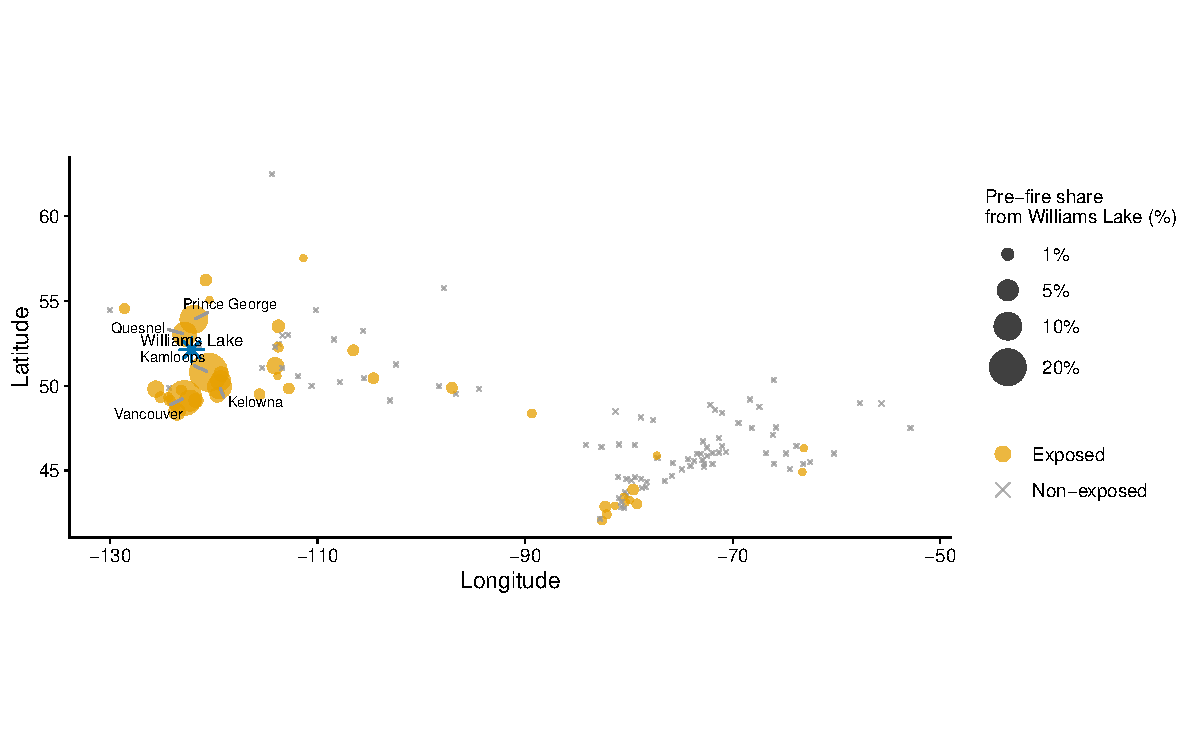
\includegraphics[width=0.60\textwidth]{figures/fig_spatial_exposure}
\end{center}

\vspace{-4pt}
{\small \textit{July 2017. Williams Lake, BC: 11,000 evacuees, $<$24 hours' notice.}
\\
\textit{Where do they go? Do rents rise there?}}

% Note: L'image suffit. Ne lis pas la légende.
%       "Ce graphique montre qui est exposé à Williams Lake."
%       Pointe les villes : Kamloops (21%), Vancouver (17%), Prince George (10%).
\end{frame}

% ============================================================
% SLIDE 4 — DESIGN D'IDENTIFICATION
% ============================================================
\begin{frame}{Identification strategy}

\textbf{Exposure index} (shift-share, continuous DiD):
\[
Z_{WL,dt} \;=\; \underbrace{s_{WL,d}}_{\text{pre-fire share}} \;\times\; \underbrace{\mathbf{1}[t \geq 2017]}_{\text{post-fire}}
\]

\smallskip
\textbf{Main regression:}
\[
\log R_{dt} \;=\; \alpha \;+\; \pi\, Z_{WL,dt} \;+\; \gamma_d \;+\; \lambda_t \;+\; \varepsilon_{dt}
\]

\smallskip
{\small
$s_{WL,d}$ = share of WL out-migrants settling in city $d$, wave 2016/2017 \\
$\gamma_d$ = city fixed effects \quad $\lambda_t$ = year fixed effects \\
Panel: 131 Canadian cities, 2008--2024. SE clustered by city.
}

% Note: L'équation est simple. Explique en français :
%       "On pèse chaque ville par ses liens migratoires avec WL avant le feu."
%       "C'est un DiD continu, pas un traitement binaire."
%       Insiste sur : les parts sont PRÉ-déterminées.
\end{frame}

% ============================================================
% SLIDE 5 — TABLE DE RÉGRESSION PRINCIPALE
% ============================================================
\begin{frame}{Main results: five specifications}

\begin{center}
\small
\begin{tabular}{lrrrrr}
\toprule
 & (1) & (2) & (3) & \textbf{(4)} & (5) \\
 & OLS & +Year FE & +City FE & \textbf{TWFE} & +City trends \\
\midrule
$Z_{WL}$ & $3.84^{***}$ & $2.49^{***}$ & $3.40^{***}$ & $\mathbf{0.818^{***}}$ & $0.594^{***}$ \\
         & (1.05)       & (0.86)       & (0.85)        & \textbf{(0.216)}  & (0.175) \\
\addlinespace
$N$ & 2,225 & 2,225 & 2,225 & 2,225 & 2,225 \\
City FE & & & \checkmark & \checkmark & \checkmark \\
Year FE & & \checkmark & & \checkmark & \checkmark \\
City trends & & & & & \checkmark \\
\bottomrule
\end{tabular}
\end{center}

{\small Dep. var.: log monthly rent, two-bedroom apartments. SE clustered by city.}

% Note: Montre la colonne (4) du doigt.
%       "Les colonnes 1-3 captent des différences structurelles.
%        La colonne 4 est notre estimation principale."
%       Laisse le tableau visible. Ne te précipite pas.
\end{frame}

% ============================================================
% SLIDE 6 — EVENT STUDY
% ============================================================
\begin{frame}{Dynamic effects: event study}

\begin{center}
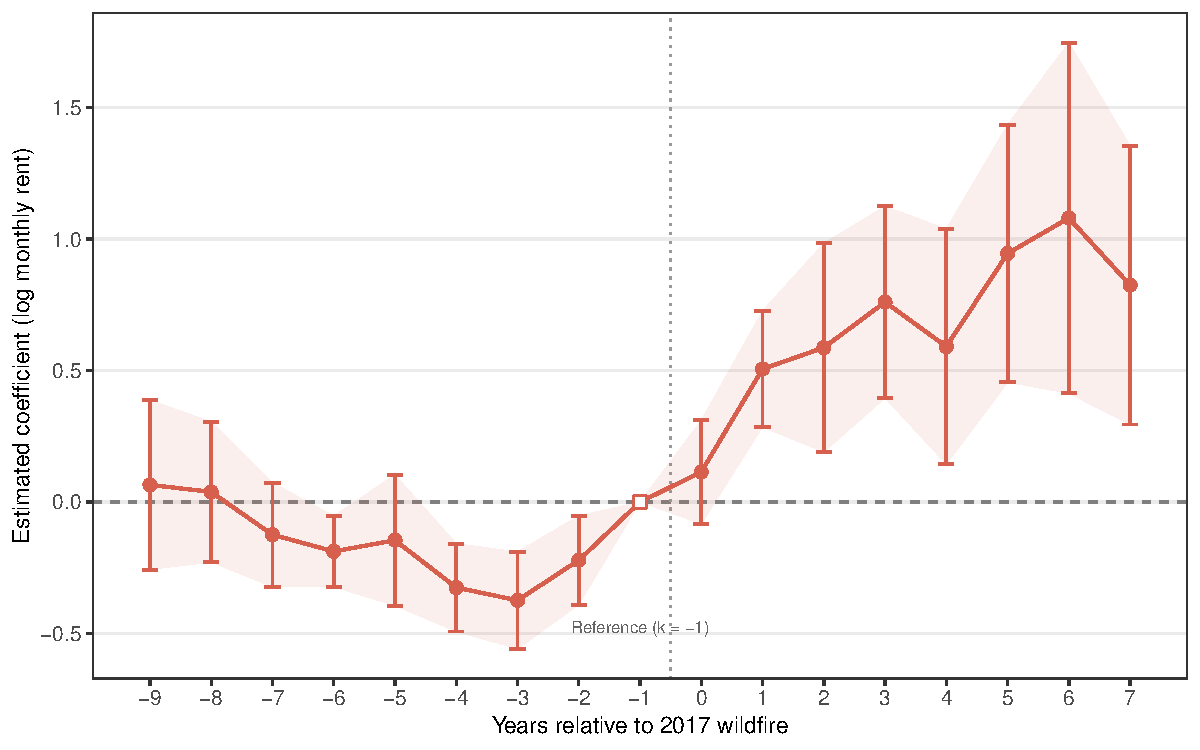
\includegraphics[width=0.78\textwidth]{figures/event_study_wl_pretrends}
\end{center}

{\small Pre-trends near zero. Coefficients grow from $k=1$ onward.
At $k=6$: $\hat{\beta}_6 \approx 1.22$ log-points ($\approx 29\%$ for Kamloops).}

% Note: "Les coefficients pré-2017 sont proches de zéro."
%       "La hausse est progressive, pas un saut immédiat — cohérent avec les baux annuels."
%       "Mais la tendance croissante post-2020 soulève la question COVID."
\end{frame}

% ============================================================
% SLIDE 7 — LE PROBLÈME D'IDENTIFICATION (province×year)
% ============================================================
\begin{frame}{The identification challenge}

\begin{center}
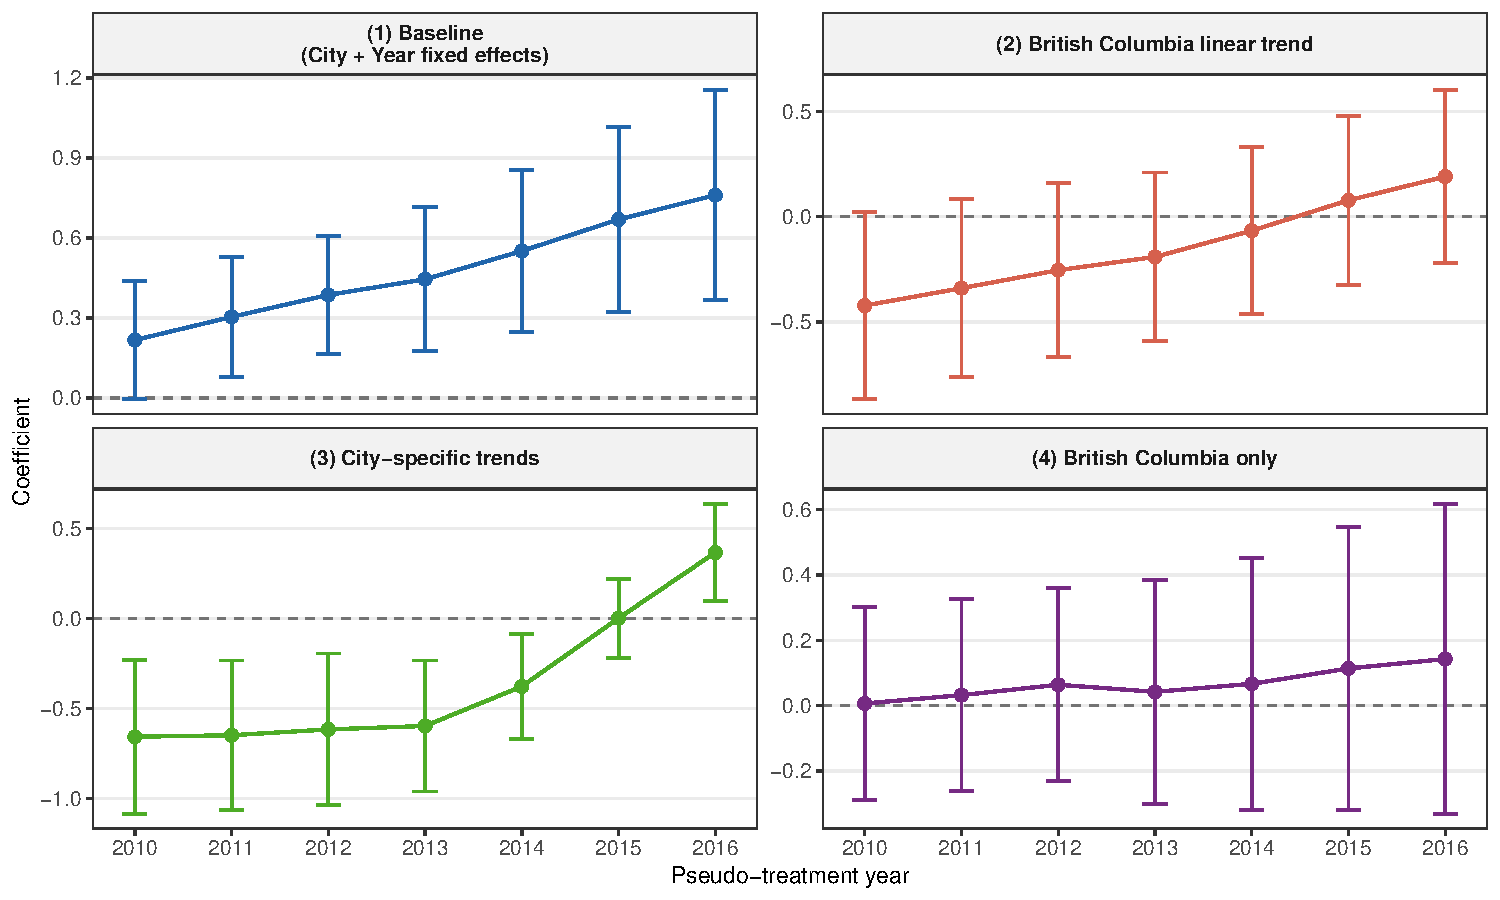
\includegraphics[width=0.78\textwidth]{figures/placebo_tests}
\end{center}

{\small \textbf{Problem:} placebo treatment years 2010--2016 produce positive coefficients in the baseline.
\\[4pt]
Province $\times$ Year FE absorbs BC dynamics: $\hat{\pi} = 0.164$ (s.e.\ $0.260$), not significant.}

% Note: "Ce graphique est la critique la plus forte."
%       "Les villes exposées croissaient DÉJÀ plus vite avant le feu."
%       "La spécification Province×Year élimine cette tendance —
%        mais aussi une partie de l'effet réel (24 villes BC seulement)."
%       Anticipe la question du jury sur les parallel trends.
\end{frame}

% ============================================================
% SLIDE 8 — LE PARADOXE SUDBURY
% ============================================================
\begin{frame}{The Sudbury result}

\begin{center}
\begin{tabular}{lcc}
\toprule
Origin & Coefficient & SE \\
\midrule
Williams Lake (pre-COVID, $\leq$2019) & $0.544^{***}$ & (0.177) \\
\textbf{Greater Sudbury} (placebo, Ontario) & $\mathbf{0.548^{***}}$ & \textbf{(0.208)} \\
Quesnel (placebo, near WL) & $0.682^{*}$ & (0.348) \\
\bottomrule
\end{tabular}
\end{center}

\bigskip
{\small Greater Sudbury: 5,000 km from Williams Lake. No wildfire. Orthogonal migration network.}

\medskip
\begin{center}
$\Rightarrow$ \textit{The design captures \textbf{migration connectivity}, not the specific wildfire event.}
\end{center}

% Note: "C'est le résultat le plus difficile à défendre."
%       "Sudbury donne le même coefficient que WL. Pourquoi ?"
%       "Réponse honnête : les loyers post-2017 sont corrélés aux réseaux migratoires
%        au sens large, pas spécifiquement au feu."
%       Écoute la question en entier avant de répondre. Ne te défends pas trop vite.
\end{frame}

% ============================================================
% SLIDE 9 — CE QU'ON APPREND (interpretation)
% ============================================================
\begin{frame}{What the data say}

\bigskip
\begin{center}
\begin{tabular}{lc}
\toprule
Test & Estimate \\
\midrule
Baseline TWFE & $0.818^{***}$ \\
Province $\times$ Year FE & $0.164$ \quad (not sig.) \\
\midrule
\textbf{Credible range} & $[0.164,\; 0.818]$ \\
\bottomrule
\end{tabular}
\end{center}

\bigskip
\begin{center}
{\small Pre-existing migration networks \textbf{predict} post-2017 rent trajectories.}\\[4pt]
{\small Provincial dynamics confound the wildfire-specific reading.}\\[4pt]
{\small Annual migration flows show \textbf{no} post-fire amplification: $-95.8^{***}$ (s.e.\ $8.9$).}
\end{center}

% Note: "On ne peut pas isoler l'effet du feu de la dynamique provinciale BC."
%       "Mais l'intervalle [0.164, 0.818] est informatif."
%       "Ce papier cartographie le terrain d'identification —
%        c'est sa contribution principale."
\end{frame}

% ============================================================
% SLIDE 10 — IMPLICATIONS ET PROCHAINES ÉTAPES
% ============================================================
\begin{frame}{Policy and next steps}

\textbf{Policy implication:}
\medskip

Disaster relief stops at the burn perimeter. Receiving cities bear housing costs
that the current framework ignores.

\bigskip
\textbf{To establish a causal estimate, the next design needs:}

\medskip
\begin{center}
\begin{tabular}{ll}
\toprule
Limitation & Solution \\
\midrule
Single origin (WL) & Multiple wildfires, multiple origins \\
BC regional confounding & Cross-provincial variation in exposure \\
Annual migration data & Higher-frequency mobility records \\
\bottomrule
\end{tabular}
\end{center}

% Note: Termine sur une note positive et concrète.
%       "La prochaine étape est claire : plusieurs feux, plusieurs provinces."
%       "Mon papier montre ce qu'on peut et ne peut pas identifier avec ce design."
%       Remercie le jury. Parle lentement à la fin.
\end{frame}

% ============================================================
% SLIDE 11 — SLIDE DE CONCLUSION (optionnel / récapitulatif)
% ============================================================
\begin{frame}{Summary}

\begin{center}
{\large \textbf{The Impact of Wildfire Evacuation on Rental Prices}}\\[6pt]
{\large Evidence from Canada --- Williams Lake, July 2017}
\end{center}

\bigskip
\begin{center}
\begin{tabular}{ll}
\toprule
Setting & 131 Canadian cities, 2008--2024 \\
Design & Continuous DiD, shift-share exposure \\
Baseline estimate & $\hat{\pi} = 0.818^{***}$ ($+19\%$ for Kamloops) \\
Credible range & $[0.164,\; 0.818]$ \\
Channel test & No migration amplification ($-95.8^{***}$) \\
Reading & Reduced-form correlation along networks \\
\bottomrule
\end{tabular}
\end{center}

\bigskip
\begin{center}
{\small Code \& data: \texttt{github.com/Robin-Economist/The-Impact-of-Wildfires-on-Rental-Prices-Evidence-from-Canada}}
\end{center}

\end{frame}

% ============================================================
% ANNEXES (hors décompte principal)
% ============================================================
\appendix

\begin{frame}{Appendix A — Heterogeneity by city size, region, supply}
\begin{center}
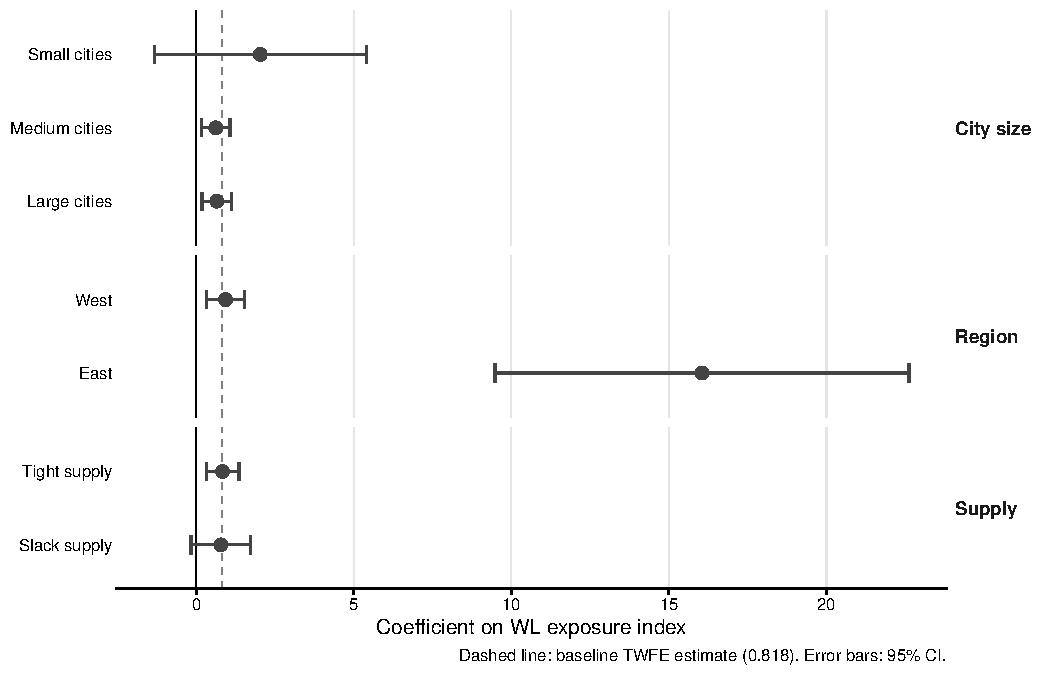
\includegraphics[width=0.82\textwidth]{figures/fig_heterogeneity_all_dims}
\end{center}
{\small 5 of 7 subgroups survive Benjamini-Hochberg correction ($q<0.05$).}
\end{frame}

\begin{frame}{Appendix B — Reduced-form scatter}
\begin{center}
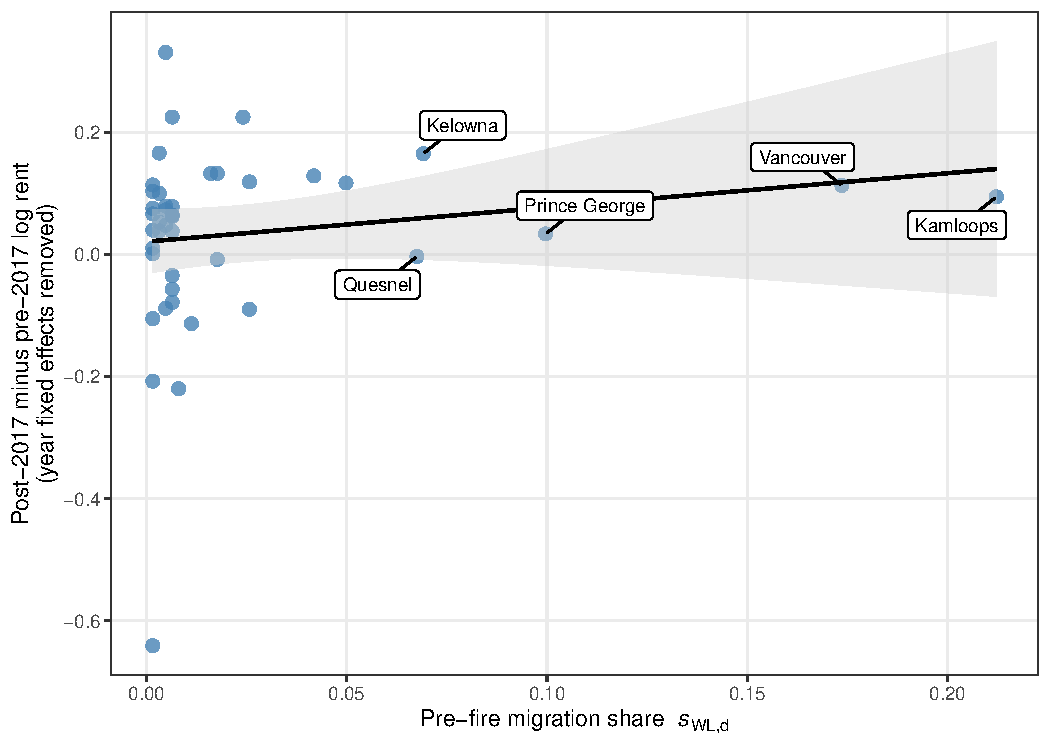
\includegraphics[width=0.70\textwidth]{figures/scatter_reducedform}
\end{center}
{\small Slope = $0.818$. Each point is an exposed city ($s_{WL,d}>0$, $N=43$).}
\end{frame}

\begin{frame}{Appendix C — Economic calibration}
\begin{center}
\small
\begin{tabular}{lrrr}
\toprule
City & Share $s_{WL,d}$ & $\Delta\%$ baseline & $\Delta$\$ baseline \\
\midrule
Kamloops      & 21.2\% & 19.0\% & \$161 \\
Vancouver     & 17.4\% & 15.3\% & \$129 \\
Prince George & 10.0\% &  8.5\% & \$72  \\
Kelowna       &  6.9\% &  5.8\% & \$49  \\
Quesnel       &  6.8\% &  5.7\% & \$48  \\
\bottomrule
\end{tabular}
\end{center}
{\small Reference rent: \$848 (national average, 2015). Baseline $\hat{\pi}=0.818$.}
\end{frame}

\begin{frame}{Appendix D — Rambachan-Roth sensitivity}
{\small Breakdown value $\bar{M}^* = 0.38$: the post-2017 confidence set
ceases to exclude zero once post-treatment trend violations reach
38\% of the largest pre-treatment deviation.}

\medskip
\begin{center}
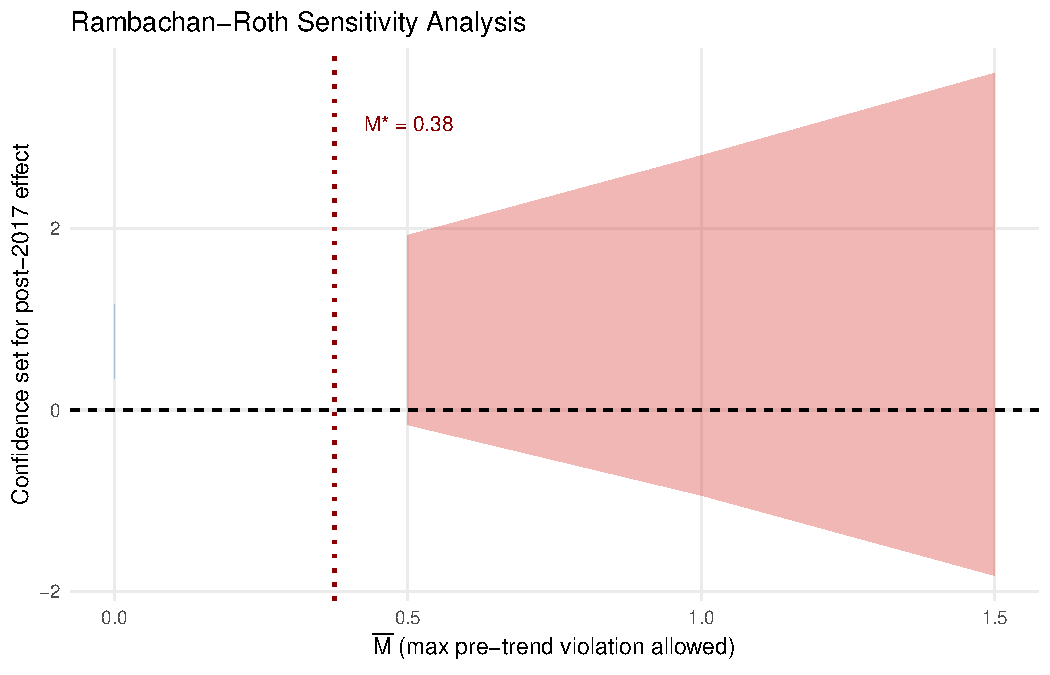
\includegraphics[width=0.70\textwidth]{figures/rambachan_roth_plot}
\end{center}
% Note: Ce slide est en annexe. Ne le présente que si on te pose la question
%       sur la sensibilité aux violations des parallel trends.
\end{frame}

\end{document}
